% !TeX root = ../main.tex

\chapter{Hilbert Space}

What is Hilbert space? and Why do we think it is important?

\begin{enumerate}
  \item A \emph{\fbox Q}\/HO (modules)
  \item A Qubit (modules)
  \item A piece of metal (real world objects)
  \item An Atom (real world objects)
\end{enumerate}
Real world objects BUILD modules

Two groups: Physics VS Math

Physics:
\begin{itemize}
  \item Stern-Gerlach 1921, 22.
  
  Silver atoms -> electron -> as spin 1/2.

  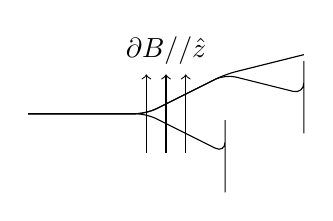
\begin{tikzpicture}
    \draw [rounded corners] (0,0) --++ (1.5,0) --++ (1,.5) --++ (1,.25);
    \draw [rounded corners] (0,0) --++ (1.5,0) --++ (1,.5) --++ (1,-.25) --++ (0,.5) --++ (0,-1);
    \draw [rounded corners] (0,0) --++ (1.5,0) --++ (1,-.5) --++ (0,.5) --++ (0,-1);
    \draw [->] (1.5,-.5) --++ (0,1);
    \draw [->] (1.75,-.5) --++ (0,1) node [above] {$\partial \bm B // \hat z$};
    \draw [->] (2,-.5) --++ (0,1);
  \end{tikzpicture}

  * Only 2 possible outcomes to fixed measurement.

  * Always 2 outcomes by changes measurements, different intensities depend on measurements.
  Orthognal states:
  \begin{itemize}
    \item Projected probability
    \item Measurement (matters!)
  \end{itemize}
\end{itemize}

Math:

Hierarchy of SPACES

Topological space -> Metric space -> Normed vector space -> Inner product space and Bonaic space -> Hilbert space
\begin{itemize}
  \item Topological space: \emph{continuity}
  \item Matrix: Sence of \emph{distance}
  \item Normed vector space (also called linear space): \emph{length} and distance (Linearity)
  \item Bonaic space: Sence of completness (limit / calcules)
  \item Inner product space: Projection/overlap (sence of not only length, but also \emph{angle})
  \item Hilbert space: all of the above.
\end{itemize}

\begin{framed}
  Vector Space
  \begin{framed}
    Inner product space (sometimes called Pre-Hilbert Space)
  \end{framed}
\end{framed}

\section{Vector space}

Vectors (u,v) \& scalors (a,b)
\begin{itemize}
  \item Vector addition ``$+$''
  \fbox{Vectors form abelian group.}
  Abelian group: 4 + 1 properties. (Closure, Identity $\identity$, Inverse (always find another elements, add to it equals to identity), Associatity ($(a+b)+c = a+(b+c)$), Commutativity ($a+b = b+a$))


  \begin{framed}
    Vectors <-> Orthogonal states
  \end{framed}

  \item Scalar multiplication ``$\times$''
  A: Associatity $a(bu) = (ab)u$, I: Identity, Distr
  $f(au+bv) = af(u) + bf(v)$.

  \begin{framed}
    Scalars <->  Projected probability (amplitudes)
  \end{framed}
\end{itemize}

\section{Inner product space}

by adding one more ~: V, F, $\braket<|>$ (Inner product): C(Conjugate symmerty: take two input $\braket<u|v> = \braket<v|u>^*$ for complex number), Li (Linear Reality: $\braket<w|au + bv> = a\braket<w|u> + b\braket<w|v>$), P (Positive definiteness: $\braket<u|v> > 0$ of $u \neq 0$.)

\begin{framed}
  Inner Project <- orthogonal, projected, measurement
\end{framed}

Operators:

Maps on Hilbert Space (linear): $Z: V \to V$

Two important defs:
\begin{itemize}
  \item Operators: compute sth. like $\ab|{\braket<u|\hat O|u>}|$
\end{itemize}

\section{Features of Hilbert space}

\begin{itemize}
  \item Main basis
  \item Maps
\end{itemize}

Hilbert Space naturally describes quantum objects: superposition; complex probability amplitudes;

\fbox{Vector space \fbox{Inner product space} ~ } \kern-1em \textrightarrow $\ket|\psi> = a\ket|u> + b\ket|v>$ \textrightarrow superposition

\fbox{IPS} \textrightarrow $\braket<u|\psi> \leftrightarrow $ complex probability amplitudes.

\begin{definition}[Basis <Mathematical definition>]\leavevmode
  \begin{itemize}
    \item Linear independence
    For a set of vectors $A = \{v_i\}$ in a vector space: If
    \[\sum_A a_i v_i = 0 \Rightarrow \forall a_i = 0\]
    then $A$ is linearly independent.
    \item Linear span:
    $span(A) = \{\sum_A a_iv_i,~ a_i \in F\}$ ($F$: Field, as complex number $F \in \mathbbm C$)

    $E = \{e_i\}$ is a basis of $V$. If
    \begin{itemize}
      \item $\{e_i\}$ is linear independence
      \item $span(\{e_i\}) = V$
    \end{itemize}
    \item Dimension of Vector space: $\dim(V) = card(E)$.
    \item Expansion of $V$ over $E$
    \[
      V = \sum a_i e_i
    \]
    This expansion is unique\footnote{}.
  \end{itemize}
\end{definition}

\begin{definition}[Orthonormal Basis]
  Use $\{\ket|\alpha>\}$ for all orthogonal states, and it satisfies
  \[
    \braket<\alpha|\alpha'> = \delta_{\alpha\alpha'}
  \]
  $\alpha$ is a lable, different labels means different states. If they are different, they are orthogonal.

  Completness condition:
  \[
    \sum_\alpha \ketbra|\alpha><\alpha| = \mathbbm I_V
  \]
  $\mathbbm I$ means identity in the Hilbert space. We call the operators like this the projector $P_\alpha$: projector to the state $\ket|\alpha>$

  Existence / construction: Gram-Schmidt orthognalization.
  $\d i = e_i - \sum_{j < i} p_j e_j$

  Expension over $\{\ket|\alpha>\}$.
  \[
    \ket|\psi> = \sum_\alpha \psi_\alpha \ket|\alpha>
  \]
  \[
    \braket<\alpha|\psi> = \sum_{\alpha '}\psi_{'\alpha'}\braket<\alpha|\alpha'>,~
    \psi_\alpha \in \mathbbm C
  \]
\end{definition}

\begin{example}
  $\alpha \to x$, $\psi_\alpha \to \psi(x)$ wavefunction

  $\alpha \to k$, $\psi(k) = \int \d x \upe^{\iu kx} \psi(x)$

  $\{\alpha\} \to \{0,1\}$, $\psi_\alpha \to (\psi_0, \psi_1)\tran$

  $\ket|0>$, $\ket|1>$.

  $\alpha \to \{(k,\sigma)\}$, $\psi_\alpha \to \psi_\sigma (k)$
\end{example}


\subsection{Change of Basis}

$\{\ket|\alpha>\} \to \{\ket|\beta>\}$

\[
  \ket|\psi> = \sum_\alpha \psi_\alpha \ket|\alpha> = \sum_\beta \psi_\beta \ket|\beta>
\]
\[
  \psi_\beta = \braket<\beta|\psi> = \sum_\alpha \braket<\beta|\alpha>\braket<\alpha|\psi> = \sum_\alpha U_{\beta\alpha} \psi_\alpha.
\]
$\beta \to k$, $\alpha \to x$
\[U_{\beta\alpha} \to \braket<k|x> = \upe^{-\iu kx}\]

\section{Maps}

Maps: just the arrow.

For vector space $(V,F)$ (sth we call vectors and scalors).

%   -> F
% V -> V
%   -> W

% Linearity (linear maps)

From $V$ to $F$: linear function

From $V$ to $V$: linear operator

Linear:

$f: V \to W$

$f(au + bv) = af(u) + bf(v)$
\[
  \{f(\text{linear}):V \to W\} = \text{Hom}_F (V,W) \text{is V.S.}
\]
\fbox{Scalor is just the one Dimension of V.S..}

$f, g \in \mathcal V$. $\forall v \in V$, $(f + g) = f(v) + g(v) \in W$.

For commutativity`', $f \cdot g = g \cdot f \in W$.

\begin{table}[!htbp]
  \centering
  \begin{tabular}{ccc}
    \toprule
    Basis & ON. Basis & Components\\
    \midrule
    $\{f_i, f_i(e_j) = \delta_{ij}\}$ & $\{\braket<\alpha|\cdot>\}$\\
    $\{f_{ij}: f_{ij}(l_n) = e_i\delta_{jk}\}$ & $\{\bra<\alpha|\}$\\
    $\{f_{ij}: f_{ij}(e_k) = e_i'\delta_{jk}\}$ & \\
    \bottomrule
  \end{tabular}
\end{table}
$\braket<\hat F|\hat G> = \sum_\alpha \braket<\hat F_\alpha|\hat G_\alpha>$
and $\hat F\ket|G> = \sum_n \braket<\alpha|\alpha>\bra<G|$
\[
  \bra<F\beta| = \sum_\alpha \braket<\beta|\alpha>\bra<\hat F_\alpha|,~
  F\ket|\beta> = \sum_\alpha \hat F \ket|\alpha>\braket<\alpha|\beta>
\]
with $\sum_\beta \ketbra|\beta><\beta| = \identity$
\[
  \sum_\beta \braket<\hat F\beta|\hat G\beta>
  = \sum_{\beta\alpha\alpha'}\braket<\beta|\alpha>\braket<F\alpha|G\alpha'>\braket<\alpha'|\beta>
\]
Then, we have
\[
  \braket<\hat F|\hat G> = \Tr(F^{-1}G) = \sum_\alpha\braket<F\alpha|G\alpha> = \sum_\alpha \braket<\alpha|F^\dagger G|\alpha>
\]
\[
  \Tr[(\ketbra|\alpha'><\alpha|)^\dagger(\ketbra|\beta><\beta'|)] = \delta_{\alpha\beta}\delta_{\alpha'\beta'}
\]
\[
  \hat O = \sum_{\alpha\beta} \ket|\alpha>\braket<\alpha|\hat O|\beta>\bra<\beta|
  = \sum_{\alpha\beta} O_{\alpha\beta}\ketbra|\alpha><\beta|
\]

How about $V \times V$? --- Inner product, a set of all pairs. It has to BILINEAR.
\[
  f(au+bv,w) = a^*f(u,w) +*b^f(v,w)
\]

$V \times V \to V \otimes V$ ($\otimes$: $V \times V \to V \otimes V$, a map)

\[w = \sum_{ij} W_{ij} (e_i \otimes e_j) = u \otimes v\]
Given $u$ and $v$, what the Components of $u \otimes v$?

Suppose $u$ is written as $u = \sum_i u_i e_i$ and $v$ is written as $v = \sum_j v_j e_j$. Then,
\[
  u \otimes v = \ab(\sum_i u_i e_i) \otimes \ab(\sum_j v_j e_j)
= \sum_i u_i (e_i \otimes \sum_j v_j e_j)
= \sum_{ij} u_iv_j (e_i \otimes e_j)
\]
We start from something like
\[
  w = w_ie_1\otimes e_1 + w_2 e_2 \otimes e_2
\]
which $w_1$ and $w_2$ are both finite.
Suppose $w = u \otimes v$ is true, then
\[
  w = \sum_{ij} u_iv_j (e_i \otimes e_j)
\]
\emph{but we have chosen a specific $w$}, it means that
\[
  w = u_1v_1(e_1 \otimes e_2) + u_1v_2(e_1\otimes e_2) + u_2v_1(e_2\otimes e_1) + u_2v_2(e_2\otimes e_2)
\]
Comparing with $w = w_ie_1\otimes e_1 + w_2 e_2 \otimes e_2$, we have
\[
  w_1 = u_1v_2, ~ 0 = u_1v_2, ~ 0 = u_2v_1, ~ w_2 = u_2v_2
\]

\subsection{Case study: (Re)discover Fourier Transform}

\begin{paracol}{2}
  We've always talk about $\{\ket|\alpha>\}$, but now,
  consider a Hilbert space, label basis $\{\ket|l>\}$ with order number index:
  \[
    \{\ket|l>,\ l = 1,\ 2,\ \ldots\,.~N\}
  \]
  and also we may want to $N + 1 \equiv 1$,
  something like a circle with all the states
  $\ket|1>$, $\ket|2>$, $\ldots\,$,~$\ket|n>$ in the right figure.

  In this basis, we define translation (operator $\hat T_L$)
  \[\hat T_L\ket|l> = \ket|l + 1>,\]
  and we may also write it differently like
  \switchcolumn \centering
  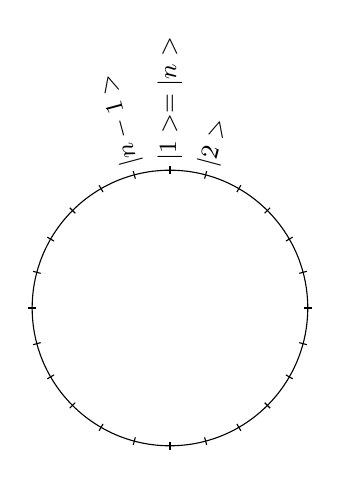
\begin{tikzpicture}[font = \small]
    \draw (0,0) circle (1.75);
    \foreach \i in {15,30,...,360}
      \draw (\i:1.7) --++ (\i:.1);
    \node [right, rotate around = {90:(0,0)}] at (90:1.75) {$\ket|1> = \ket|n>$}
     node [right, rotate around = {75:(0,0)}] at (75:1.75) {$\ket|2>$}
     node [right, rotate around = {105:(0,0)}] at (105:1.75) {$\ket|n - 1>$};
  \end{tikzpicture}
\end{paracol}
\begin{equation}
  \hat T_L = \sum_l \ketbra|l + 1><l|,
\end{equation}
The eigenvalue
\[
  \hat T_L\ket|\psi> = \lambda \ket|\psi>
\]
while $\ket|\psi> = \sum_l \psi_l \ket|l>$, that is
\begin{align*}
  \hat T_L\ket|\psi>  & = \sum_l \psi_{l-1}\ket|l>\\
  \lambda\ket|\psi>   & = \sum_l \lambda \psi_l \ket|l>
\end{align*}
Then we have
\[
  \psi_l = \lambda \psi_l, ~ \psi_l = \lambda^{1-l}\psi_l,~
  \psi_1 = \psi_{N+1} = \lambda^{-N}\psi_1
\]
then we have $\lambda^{-N} = 1$. So, we can specify $\lambda$
\begin{equation}
  \lambda = \lambda_m \equiv \upe^{-\iu \frac{2\pi}Nm}
\end{equation}
Concering the eigenstates of $\hat T_L$, which are $\ket|m>$. Since
\[
  \psi_{1,m} = \lambda_m^{-1}, ~ \psi_{l,m} = \lambda_m^{1-l}\psi_{1,m} = \lambda_m^{-l}
\]
So,
\[
  \ket|m> = \sum_l \psi_{l,m}\ket|l> = \frac1{\sqrt N} \sum\upe^{\iu \frac{2\pi}{N} ml} \ket|l>
\]
Now, consider the new basis ($m = 1$, $2$, $\ldots\,$,~$N$), 
the relation between it and the old basis is
\[
  \{\ket|l>\} \xleftrightarrow{\text{Fourier Transform}} \{\ket|m>\}
\]
In this basis, the definition of the operator is
\begin{equation}
  \hat T_L = \sum_m \upe^{-\iu \frac{2\pi}{N}m} \ketbra|m><m|.
\end{equation}
with $N + 1 \equiv 1$.
and the inner product
\begin{equation}
  \braket<l|m> = \frac1{\sqrt N}\upe^{\iu\frac{2\pi}{N}lm}
\end{equation}
To make the problem more interesting: the translation of the $m$-basis,
express $\hat T_M$ in terms of $l$
\begin{equation}
  \hat T_M = \sum_m \ketbra|m + 1><m|
= \sum_{mll'} \ket|l>\braket<l|m+1>\braket<m|l'>\bra<l|
\end{equation}
If we put $m + 1$ instead of $m$
\[
  \braket<l|m + 1> = \upe^{\iu\frac{2\pi}{N}l} \braket<l|m>
\]
subsitute it into $\hat T_M$
\[
  \hat T_M = \sum_l \upe^{\iu\frac{2\pi}{N}l}\ketbra|l><l|
\]
To summarize
\begin{align}
  \hat T_L & = \upe^{-\iu\frac{2\pi}{N}\hat M}, ~
  \hat M = \sum_m m\ketbra|m><m|\\
  \hat T_M & = \upe^{-\iu\frac{2\pi}{N}\hat L}, ~
  \hat M = \sum_m m\ketbra|l><l|
\end{align}
This is only a start. How about the translation over $m$:
\[
  \hat T_L \hat T_M = \underline? \hat T_M \hat T_L,
\]
means we can measure $M$ first, then measure $L$; or reverse.
They will differ by something like
\[
  \hat T_M \hat T_L = \hat T_L \hat T_M \upe^{\iu\frac{2\pi}{N}}
\]
Comparing with $[\hat q,\hat p] = \iu$.
Just consider in the $l$ basis, expand $\hat T_L$ and $\hat T_M$
\begin{align*}
  \hat T_L \hat T_M & = \sum_{ll'} \ketbra|l + 1><l| \upe^{\iu\frac{2\pi}{N}l'}\ketbra|l'><l'|
= \sum_l \upe^{\iu\frac{2\pi}{N}l}\ketbra|l + 1><l|\\
  \hat T_M \hat T_L & = \sum_{ll'} \upe^{\iu\frac{2\pi}{N}l'} \ket|l'>\braket<l'|l + 1>\bra<l|
= \sum_l \upe^{\iu\frac{2\pi}{N}(l+1)} \ketbra|l + 1><l|
\end{align*}
That is
\begin{equation}
  \hat T_M \hat T_L = \upe^{\iu\frac{2\pi}{N}}\hat T_L \hat T_M
  \label{1.7}
\end{equation}
When $N = 2$: we reach \emph{Ultra Quantum};
When $l = 0$, $1$: $\hat T_M \to \sigma_z$, and $\hat T_L \to \sigma_x$.
We get the anti-commute relation
\begin{equation}
  \sigma_z \sigma_x = -\sigma_x\sigma_z
\end{equation}
When $N \to \infty$, $q = la$ while $a \to 0$,
similarly, $p = mb = m\frac{2\pi}{Na}$. Eventually, $b \to 0$, $N \to \infty$.

Let $\hat Q = \hat La$, $\hat P = \hat Mb$, now
\[
  \hat T_M \to \hat T_Q = \upe^{\iu b\hat Q}, \qq{and}
  \hat T_L \to \hat T_P = \upe^{-\iu a\hat P}
\]
Next, what we need to do is to expand the exponential to linear order: from \eqref{1.7}, we have
\[
  (\identity + \iu b\hat Q) (\identity - \iu a\hat P)
= (\identity + \iu ab) (\identity - \iu a\hat P) (\identity + \iu b\hat Q)
\]
Omit the high order terms, then we have
\begin{equation}
  \hat Q \hat P = \iu + \hat P \hat Q, \qq{or} [\hat Q, \hat P] = \iu
\end{equation}
$Q$ and $P$ are Hermitian Operators.

\noindent\rule{\linewidth}{1pt}

\[
  \hat O\ (V \to V)
  \begin{cases*}
    \text{Invertible:} &
    Symmetry Operators (e.g. projection: $\ketbra|\alpha><\alpha|$ or $\sum_{\{\alpha\}\in \text{H.S.}} \ketbra|\alpha><\alpha|$)\\
    & Transformation, time evolution: Unitary $U^\dagger U = \identity$\\
    \text{Non-Invertible:} & Generators \texttt{<->} Obserables\\
    & Hamiltonian, position \texttt{<->} momentum: Hermitian $O^{-1} = O$
  \end{cases*}
\]
For any $\Psi X \Psi$, the unitary operation should satisfy the following relation
\begin{equation}
  \braket<\hat UX|\hat O\Psi> = \braket<X|\Psi>
\end{equation}
while the Hermitian operator should satisfy
\begin{equation}
  \braket<\hat OX|\Psi> = \braket<X|\hat O\Psi>
\end{equation}
Another kind of unitary: Anti-Unitary \texttt{<-} Anti-Linear

\section{Time Evolution}

\[\ket|\Psi(t)> = \hat U(t,t_0) \ket|\Psi(t_0)>\]
\[
  \braket<\hat O\Psi(t_0)|\hat O\Psi(t_0)> = \braket<\Psi(t_0)|\Psi(t_0)>
\]

The two statements: Operator $\hat O$ satisfies
\begin{itemize}
  \item $\forall \psi$, $\braket<\hat O\psi|\hat O\psi> = \braket<\psi|\psi>$ (Preserve norm)
  \item $\forall X, \psi$, $\braket<\hat OX|\hat O\psi> = \braket<X|\psi>$ 
  (Preserve inner product)
\end{itemize}
Prove that they are equivalent.
\begin{proof}
  Obviously, 2 to 1 is trivial.
  Let $u = X + \Psi$, $V = X + \iu\Psi$, then subsitute them in to the above formulas.
\end{proof}

\subsection{Equation of Motion}

$\hat U$: linear, continous with time.

We need to consider $\epsilon$ time difference, that is somethint like
\[
  \ket|\Psi(t + \epsilon)> = \hat U(t + \epsilon, t) \ket|\Psi(t)>
\]
\[
  \lim_{\epsilon\to0}
  \frac{\ket|\Psi(t+\epsilon)> - \ket|\Psi(t)>}{\epsilon}
= \lim_{\epsilon\to0} \frac{\hat U(t + \epsilon,t) - \hat U(t,t)}{\epsilon} \ket|\Psi(t)>
\]
\[
  \text{LHS} = \odv*{\ket|\Psi(t)>}t, ~
  \lim_{\epsilon\to0} \frac{\hat U(t + \epsilon,t) - \hat U(t,t)}{\epsilon}
= \odv*{}{t} \hat U(t',t)\bigg|_{t'=t} \equiv \frac1{\iu\hbar} \hat H(t)
\]
Finally, we approach the Schr\"odinger Equation
\begin{equation}
  \odv*{\ket|\Psi(t)>}t = \frac1{\iu\hbar} \hat H(t) \ket|\Psi(t)>
\end{equation}
Prove: $\hat g$ is Hermitian
\begin{equation}
  \odv*{\hat U(\theta)}\theta \bigg|_{\theta=0} = \iu \hat g
\end{equation}
while $\hat U(0) = \identity$.
\begin{proof}
  We know that 
  \[\hat U(\epsilon) = \identity + \iu \hat g\epsilon\]
  Since the definition of Hermitian is
  \[
    \braket<\hat OX|\Psi> = \braket<X|\hat O\Psi>,
  \]
  Then plug $\hat U(\epsilon)$ into the definition
  \[
    \braket<\hat U(\epsilon)X|\hat U(\epsilon)\Psi>
  = \braket<X|\psi> + (-\iu\epsilon)\braket<\hat gX|\Psi>
  + (\iu\epsilon)\braket<X|\hat g\Psi> = \braket<X|\Psi>
  \]
  then we have
  \[
    \braket<\hat gX|\Psi> = \braket<X|\hat g\Psi>
  \]
  means that $\hat g$ is Hermitian.
\end{proof}
$\hat g$ is called the generator; \emph{$\hbar$ / Hamiltonian is the generator of time evolution.}
\begin{equation}
  \iu\odv*{\ket|\Psi(t)>}t = \hat H(t) \ket|\Psi(t)>
\end{equation}
$\hat H$ is canonical quantization. Replace $\ket|\psi(t)>$
\begin{equation}
  \iu\odv*{\hat U(t,t_0)}t = \hat H(t) \hat U(t,t_0)
\end{equation}
Given $\hat H(t)$, find $\hat U(t_f,t_i)$. For t-independent $\hat H$, do small steps from $t_i$ to $t_f$ by $\delta t = (t_f - t_i)/N$
\begin{equation}
  \hat U(t_f,t_i) = \hat U(t_f,t_f - \delta t) \hat U(t_f - \delta t, t_f - 2\delta t) \ldots \hat U(t_i + \delta t, t_i)
\end{equation}
When $N \to \infty$, $\delta t \to 0$, that become
\[
  \hat U(t_f,t_i) = \lim_{N\to\infty}  (\identity - \iu \hat H \delta t)^N
= \lim_{N\to\infty} \ab(\identity - \iu \hat H \frac{t_f - t_i}{N})^N
= \upe^{-\iu\hat H(t_f - t_i)}
= \identity + ()\hat H + ()\hat H^2 + \cdots
\]

\subsection{Dyson series}

When it's time-independent, the order doesn't matter.
Now, consider the $t$-dependent case of $\hat H(t)$
\[
  \hat U(t_f,t_i) = \lim_{\delta t\to0}
                    (\identity - \iu \hat H(t_f)\delta t)
                    (\identity - \iu \hat H(t_f - \delta t)\delta t)
                    \cdots
                    (\identity - \iu \hat H(t_i + \delta t)\delta t)
\]
and convert every term into exponential $\upe^{-\iu\hat H(t_i + \delta)\delta t}$, the first term gets $\upe^{-\iu\hat H(t_f)\delta t}$. Multiply all the exponential function, $\upe^{-\iu\int_{t_i}^{t_f} \d t \hat H(t)}$.
\begin{framed}
  Since $\upe^A\upe^B \sim \upe^C$, but $C = A + B + ()[A,B] + \cdots$.
  And a time ordering operator $\mathcal T$ is applied before the exponential.
\end{framed}
Now, rewrite the S.E
\begin{equation}
  \int_{\mathemph{t_i}}^{t_f} \d \hat U(t,\mathemph{t_i})
= \int_{t_i}^{t_f} [-\iu\hat H(t)] \hat U(t,t_i) \d t
\end{equation}
since the lower limit of the integral $t_i$
and the second time variable of $\hat U$: $t_i$ conduct an identity, that is
\[
  \text{LHS} = \hat U(t_f,t_i) - \hat U(t_i,t_i) = \hat U(t_f,t_i) - \identity
\]
so
\begin{align*}
  \hat U(t_f,t_i) & = \identity + \int_{t_1}^{t_f} \d t_1
                    [-\iu \hat H(t)] \hat U(t_1,t_i)\\
& = \identity + \int_{t_1}^{t_f} \d f_1 (-\iu \hat H(t_1))
  + \int_{t_i}^{t_f} \d t_1 (-\iu \hat H(t_1)) \int_{t_i}^{t_1} \d t_2
    (-\iu\hat H(t_2))\\
& + \cdots + \int_{t_i}^{t_f} \d t_1 + \int_{t_i}^{t_1} \d t_2 \cdots
  + \int_{t_i}^{t_{n-1}} \d t_n (-\iu \hat H(t_1)) \cdots (-\iu\hat H(t_N)) + \cdots
\end{align*}
That's what we called the \emph{Dyson's Series}.
Now, let's take a look at $N$'s order term
\begin{multline}
  \int_{t_i}^{t_f} \d t_1
  \int_{t_i}^{\mathemph{t_1}} \d t_2
  \cdots
  \int_{t_i}^{\mathemph{t_{n-1}}} \d t_n
  \hat H(t_1) \hat H(t_2) \cdots \hat H(t_n)
= \int_{t_i}^{t_f} \d t_1
  \int_{t_i}^{\mathemph{t_f}} \d t_2
  \int_{t_i}^{\mathemph{t_f}} \d t_n\\
  \theta(t_1 - t_2) \cdots \theta(t_{n-1} - t_n)
  \hat H \cdots \hat H
\end{multline}
while
\begin{equation}
  \theta(x) =
  \begin{cases}
    1, & x > 0\\
    0, & x < 0
  \end{cases}
\end{equation}
is the Heaviside Stage Function. It could
\begin{equation}
  \int_{x_0}^{x_1} \d x = \int_{x_0}^{\infty} \d x \theta(x_0 - x)
\end{equation}
\begin{center}
  \begin{tikzpicture}
    \draw (0,0) node [below] {$x_0$} -- (2,0) node [below] {$x_1$} -- (5,0)
     node [below] {$\infty$};
  \end{tikzpicture}
\end{center}
$t_1$, $t_2$, $\ldots$, are Dummy variables.
Then, sum over all of the  permutations
\begin{align*}
  & \int_{t_i}^{t_f} \d t_1
  \int_{t_i}^{\mathemph{t_f}} \d t_2
  \int_{t_i}^{\mathemph{t_f}} \d t_n
  \theta(t_1 - t_2) \cdots \theta(t_{n-1} - t_n)
  \hat H \cdots \hat H\\
  = & \frac1{n!} \sum_\sigma
  \int_{t_i}^{t_f} \d t_{\sigma_1}
  \int_{t_i}^{t_f} \d t_{\sigma_2}
  \cdots
  \int_{t_i}^{t_f} \d t_{\sigma_n}
  \theta(t_{\sigma_1} - t_{\sigma_2}) \cdots
  \theta(t_{\sigma_{n-1}} - t_{\sigma_n})
  \hat H(t_{\sigma_1}) \cdots
  \hat H(t_{\sigma_n})\\
  = & \frac1{n!}
  \int_{t_i}^{t_f} \d t_1
  \int_{t_i}^{t_f} \d t_2
  \cdots
  \int_{t_i}^{t_f} \d t_{\sigma_n} \sum_\sigma[
  \theta(t_{\sigma_1} - t_{\sigma_2}) \cdots
  \theta(t_{\sigma_{n-1}} - t_{\sigma_n})
  \hat H(t_{\sigma_1}) \cdots
  \hat H(t_{\sigma_n})]\\
\equiv & \mathcal T[\hat H(t_1) \cdots \hat H(t_n)]
= \mathemph{\frac1{n!} \mathcal T \ab[\int_{t_i}^{t_f} \d t \hat H(t)]^n}
\end{align*}
while $\sigma: \{1,2,\ldots,n\} \to \{1,2,\ldots,n\}$ is called permutation:
E.g., $\sigma_2$: $1$, $2$, $3 \to 3$, $1$, $2$.
And we introduced the time ordering operator $\mathcal T$ to prevent a Hamiltonian operator with an latter time $\hat H(t_j)$
``knocked'' on $\ket|\Psi(t)>$ earlier that
a Hamiltonian operator with an earlier time $\hat H(t_i)$ will ``knock on'':
that is
$\hat H(t_i) \hat H(t_j) \ket|\Psi(t)>$.

\section*{Review: Time Evolution}

The Schr\"odinger equation
\begin{equation}
  \iu \odv*{\ket|\psi(t)>}t = \hat H(t) \ket|\psi(t)>
\end{equation}
and we can rewrite it in terms of time-evolution operator
\begin{equation}
  \iu \odv*{\hat U(t,t_0)}t = \hat H(t) \hat U(t,t_0)
\end{equation}
and initially, we can write
\[
  \hat H(t) = \iu \odv*{\hat U(t',t)}t \bigg|_{t'=t}
= \iu \ab[\odv*{\hat U(t,t_0)}t] \hat U^{-1}(t,t_0)
\]
the bracket can be generalize something like
\begin{equation}
  \hat g_\theta = \iu \odv*{\hat U(\theta)}\theta \bigg|_{\theta=0}
\end{equation}
and we can have the identity
\begin{equation}
  \hat U(0) = \identity
\end{equation}
In general, the expression of the time-evolution operator is something like
\[
  \hat U(t,t_0) = \mathcal T \upe^{-\iu \int_{t_0}^t \d t' \hat H(t)}
\]
The time-ordering operator is inserted since
\[\upe^A \upe^B = \upe^C \neq \upe^{A+B}\]
BCH formula will tell how to write $C$:
\[
  C = A + B + \frac12[A,B] + \cdots
\]
The time-ordering operator can be also separate into two cases
\[
  \begin{cases*}
    \hat U(t,t_0) = \upe^{-\iu (t-t_0) \hat H}, & time-independent\\
    \hat U(t,t_0) = \identity + (-\iu) \int_{t_0}^t \d t_1 \hat H(t_1)
                  + (-\iu) \int_{t_0}^t \d t_1 \int_{t_0}^{t_1} \d t_2
                    \hat H(t_1) \hat H(t_2) + \cdots, & time-dependent
  \end{cases*}
\]

\subsection{Three Pictures}

Considering representation, the basis $\{\ket|\alpha>\}$.
and in state and operator
\begin{gather}
  \ket|\psi> = \sum_\alpha \psi_\alpha \ket|\alpha>\\
  \hat O = \sum_{\alpha\beta} \hat O_{\alpha\beta} \ketbra|\alpha><\beta|
\end{gather}
where $\psi_\alpha = \braket<\alpha|\psi>$ and $O_{\alpha\beta} = \braket<\alpha|\hat O|\beta>$.

\begin{itemize}
  \item Schr\"odinger: $\{\ket|\alpha>^S = \ket|\alpha>\}$, where $\ket|\alpha>$ is const in time.
  \[
    \odv*{\psi_\alpha^s(t)}t = \odv*{^s\braket<\alpha|\psi(t)>}t
  = (-\iu) ^s\braket<\alpha|\hat H(t)|\psi(t)> = \sum_\beta (-\iu) H_{\alpha} (t) \psi_\beta^s (t)
  \]
  when $\alpha \to x$, $\psi_\alpha(t) = \psi(x,t)$
  \[
    \iu \pdv*{\psi(x,t)}t = \int \d x' H(x,x',t) \psi(x',t)
    \to H(x,-\iu\pdif x, t) \psi(x,t)
  \]
  the propotion $H(x,x',t) $ is something like $\delta(x - x')$.
  \item Heisenberg
  \[
    \{\ket|\alpha(t)>^H = \hat U(t,t_0) \ket|\alpha(t_0)>\}
  \]
  for the state,
  \begin{equation}
    \odv*{\psi_\alpha^H(t)}t = \odv*{^H\braket<\alpha(t)|\psi(t)>}t = 0
  \end{equation}
  means the state is not moving at all.
  Assume $\alpha(t_0) = \alpha$, $\hat U(t,t_0) = \hat U(t)$, and $\psi(t_0) = \psi$.
  \[
    \odv*{O_{\alpha\beta}^H(t)}t = \odv*{^H\braket<\alpha(t)|\hat O|\beta(t)>^H}t = \odv*{\braket<\alpha|\hat U^{-1}(t) \hat O \hat U(t)|\beta>}t
  \]
  where $\hat U^{-1}(t) \hat O \hat U(t) = \hat O^H(t)$. Then
  \[
    \odv*{\hat O^H(t)}t = \odv*{(O^{-1}(t) \hat O \hat U(t))}t
  \]
  where $\odv*{\hat U^{-1}(t)}t = \iu \hat U^{-1}(t) \hat H(t)$.
  Finally, we have
  \begin{equation}
    \odv*{\hat O^H(t)}t = \iu[\hat H^H(t), \hat O^H(t)]
  \end{equation}
  which is so called the Heisenberg equation (EOM), where
  \[
    \hat H^H(t) = \hat U^(t)^{-1} \hat H(t) \hat U(t)
  \]
  \item Interaction
  
  We have two part of Hamiltonian
  \[
    \hat H = \hat H_0 + \hat V
  \]
  what is important is that $\hat H_0$ is the easy part,
  we can easily compute the time evolution $\hat U_0(t)$.
  Then, the basis will be chosen as
  \[
    \{\ket|\alpha(t)>^I = \hat U_0(t) \ket|\alpha>\}
  \]
  then
  \begin{equation}
    \odv*{\psi_\alpha^I(t)}t = \odv*{^I\braket<\alpha(t)|\psi(t)>}t
  = \odv*{\braket<\alpha|\hat O^{-1} \hat U(t)|\psi>}t.
  \end{equation}
  and we consider $\hat O^{-1} \hat U(t)\ket|\psi> = \ket|\psi(t)>^I$.
  Similarly,
  \begin{align*}
    \odv*{\ket|\psi_\alpha(t)>^I}t &
  = \iu \hat U_0^{-1} (\hat H_0(t) - \hat H(t)) \hat U(t) \ket|\psi>
  = \odv*{(\hat U_0^{-1} \hat U(t) \ket|\psi>)}t (?)\\ &
  = -\iu \hat U_0^{-1}(t) \hat V(t) \hat U_0(t) \hat U_0^{-1}(t) \hat V(t) \ket|\psi>
  = -\iu \hat V^I(t) \ket|\psi(t)>^I
  \end{align*}
  where $\hat U_0^{-1}(t) \hat V(t) \hat U_0(t) = \hat V^I(t)$ and
  $\hat U_0^{-1}(t) \hat V(t) \ket|\psi> = \ket|\psi(t)>^I$,
  and $\hat O(t) = \hat U_0^{-1}(t) \hat O \hat U_0(t)$.
  \[
    \odv{\hat O^I(t)}t = \iu [\hat H_0^I(t), \hat O^I(t)]
  = \odv*{(\hat U_0^{-1}(t) \hat O \hat U_0(t))}t
  \]
\end{itemize}

\hrule

\paragraph{Quiz 4}

\begin{problem}
  Given
  \[
    \odv*{\hat U_0(t,t_0)}t = -\iu \hat H_0(t) \hat U_0(t,t_0),
  \]
  show that
  \[
    \odv*{\hat U_0^{-1}(t,t_0)}t = \iu \hat U_0^{-1}(t,t_0) \hat H_0(t).
  \]
\end{problem}
\begin{solution}
  
\end{solution}

\begin{problem}
  Given
  \[
    f(z) = \upe^{-\frac12(x-z)^2}, \quad (x \in \mathbb R,~ z \in \mathbb C)
  \]
  compute
  \[
    \int_{-\infty}^{+\infty} |f(x)|^2 \d x.
  \]
\end{problem}
\hrule

\subsection{Case study}

\begin{enumext}[wrap-label = \underline{Case #1}, label = \arabic*,
                list-indent = 0pt]
  \item Quantum Harmonic Oscillator\\
  Certainly, this is a time-independent problem, the Hamiltonian is given as
  \[
    \hat H = \frac{\hat p^2}{2m} + \frac12 m\omega^2 \hat X^2.
  \]
  For simplifaction, we define $l_0 = \sqrt{\frac\hbar{m\omega}}$, then
  \[
    \hat X = \frac{\hat x}{l_0}, \qq{and} \hat k = \frac{\hat p l_0}\hbar.
  \]
  So, the original commutation relation becomes
  \[
    [\hat x, \hat p] = \iu\hbar \longrightarrow [\hat x, \hat k] = \iu.
  \]
  Certaily, we need
  \[
    \hat a = \frac1{\sqrt2} (\hat x + \iu\hat k), \qq{and}
    [\hat a, \hat a^\dagger] = 1
  \]
  and let $\hbar = 1$. Then
  \[
    \hat H = \omega(\hat a^\dagger \hat a + \frac12)
  \]
  where $\hat a^\dagger \hat a = \hat N$, the number operator.
  \begin{enumext}
    \item The eigenstates
    $\ket|n> = \frac1{\sqrt{n!}} (\hat a^\dagger)^n \ket|0>$, and
    $\hat a \ket|0> = 0$.
    Consider
    \[
      \ket|n(t)> = \hat U(t) \ket|n> = \upe^{-\iu\omega(n+\frac12)t} \ket|n>
    \]
    Then
    \[
      \braket<n(t)|\hat x|n(t)> = 0, \qq{and} \braket<n(t)|\hat k|n(t)> = 0
    \]
    where
    \[
      \hat x = \frac1{\sqrt2}(\hat a + \hat a^\dagger),
      \hat k = \frac1{\sqrt2\iu} (\hat a - \hat a^\dagger)
    \]
    In Heisenberg picture
    \[
      \dot{\hat x}(t) = \iu[\hat H(t), \hat x(t)] = \omega \hat k(t), \qq{and}
      \dot{\hat k}(t) = \iu[\hat H, \hat k(t)]    = -\omega \hat x(t)
    \]
    and we have
    \[
      \dot{\hat a}(t) = -\iu\omega\hat a(t) \Rightarrow
      \hat a(t) = \upe^{-\iu\omega t} \hat a
    \]
    \[
      \hat x(t) =  \cos\omega t \hat x + \sin\omega t \hat k,
      \hat k(t) = -\sin\omega t \hat x + \cos\omega t \hat k.
    \]
    \item Coherent States $\{\ket|\alpha>\}$
    \begin{gather*}
      \hat a \ket|\alpha> = \alpha \ket|\alpha>, ~ \alpha \in \mathbb C\\
      \ket|\psi> \sim \sum_\alpha \psi_\alpha \ket|\alpha>,~ 
      \ket|\psi(t)> = \sum_\alpha \psi_\alpha \ket|\alpha(t)>\\
      \hat a(-t) \ket|\alpha(t)> = \alpha \ket|\alpha(t)>,~
      \hat U^{-1} \hat a \hat I^{-1}(-t) \hat U(t) \ket|\alpha>\\
      \upe^{\iu\omega t} \hat a\ket|\alpha(t)> = \alpha \ket|\alpha(t)>
      \Rightarrow \alpha(t) = \upe^{-\iu\omega t} \alpha
    \end{gather*}
    What if $\ket|x(t)>$, or in other words $\ket|\psi>$ is $\ket|x_0>$
    \[
      \braket<\alpha|x_0> = \int_{x_0} (\alpha)
    \]
    \[
      \ket|\alpha> = \sum_n^\infty f_{\alpha,n} \ket|n>
    \]
    while
    \[
      \hat a\ket|\alpha> = \sum_n f_{\alpha,n} \sqrt n \ket|n - 1>
    = \sum_n f_{\alpha, n+1} \ket|n>
    \]
    where
    \[
      f_{\alpha, n+1} = \frac{\alpha}{\sqrt{n+1}} f_{\alpha,n},
      \quad
      f_{\alpha.n} = \frac{\alpha^n}{\sqrt{n!}} f_{\alpha,0}
    \]
    and
    \[
      \ket|\alpha> = N \sum_n \frac{\alpha^n}{\sqrt{n!}} \ket|n> = N \upe^{\alpha} a^{n-1} \ket|0>, \quad \ket|n> = ...
    \]
    Concering $\braket<x|\alpha>$: since
    \[
      \alpha f_\alpha(x) = \braket<x|\hat a|\alpha>
    = \int \d x' \braket<x|\hat a|x'> \braket<x'|\alpha>
    \]
    substitute $\hat a = \frac1{\sqrt 2} (\hat x + \hat k)$
    \[
      \alpha f_\alpha(x) = \frac1{\sqrt2} (x + \pdif x) f_\alpha(x)
    \]
    and
    \[
      f_\alpha(x) = N \upe^{-\frac12(x - \sqrt 2a)^{\frac\alpha2}}
    \]
    where $|f_\alpha(x)|^2 = \frac1{\sqrt\pi}\upe^{-(x-\sqrt2\alpha_x)^2}$
  \end{enumext}
  \item Rabi Problem\\
  The Hamiltonian
  \[
    \hat H(t) =
    \begin{pmatrix}
      \frac\Omega2 & \gamma\upe^{-\iu\omega t}\\
      \gamma \upe^{\iu\omega t} & -\frac\Omega2
    \end{pmatrix}
  \]
  bascially time-dependent.
  $\frac\Omega2$ and $-\frac\Omega2$ means the gap between $\ket|0>$ and
  $\ket|1>$ is $\Omega$; and driver frenquency $\omega$, intensity $\gamma$.
  \[
    U(t) =
    \begin{pmatrix}
      \ket|0> \to \ket|0> & \ket|1> \to \ket|0>\\
      \ket|0> \to \ket|1> & \ket|1> \to \ket|1>
    \end{pmatrix}
  \]
  Compute $H_0 = \pdiagmat{\frac\omega2, -\frac\omega2}$.

  Firstly, the definiton of $U_0(t)$.
  Normally, $U_0(t) = \upe^{-\iu tH_0}$; In this case
  \[
    U_0(t) = \pdiagmat{\upe^{-\iu\frac\omega2t}, \upe^{\iu\frac\omega2t}}
  \]
  and
  \[
    U_0^{-1}(t) H(t) U_0(t)
  = \begin{pmatrix}
      \frac\Omega2 & \gamma \\ \gamma & -\frac\Omega2
    \end{pmatrix},~
    V =
    \begin{pmatrix}
      \frac{\Omega - \omega}2 & \gamma\\
      \gamma & -\frac{\Omega - \omega}2
    \end{pmatrix}
  \]
  We get a matrix equation
  \[
    \iu \odv*{U(t)}t = V U(t)
  \]
  the solution is
  \[
    U(t) = \cos Delta_\omega t - \iu \sin\Delta_\omega t
    \ab(\cos\theta_\omega \sigma_z + \sin \theta_\omega \sigma_x)
  \]
  where
  \[
    \Delta_\omega = \sqrt{\ab(\frac{\Omega - \omega}{2})^2 + r^2}, \quad
    \tan \theta_\omega = \frac{2\gamma}{\Omega - \omega}
  \]
  and
  \[
    P_{0\to1}(t) = \frac{\gamma^2}{\ab(\frac{\Omega - \omega}{2})^2 + \gamma^2} \sin^2(\Delta_\omega t)
  \]
  probability: Center: $\Omega$, and $\gamma$ (coupling strength), giving a width. It's very small, means the peek is sharp;
  If $\gamma$ is large, ...
\end{enumext}